
\chapter{An Online Vector Error Correction Model for Exchange Rates Forecasting}


The Vector Error Correction Model (VECM) is an econometric model which
characterises the joint dynamic behaviour of a set of cointegrated variables in
terms of forces pulling towards equilibrium. In the previous proposal, the
Adaptive VECM (AVECM) showed that to be able to use VECM at every time step can
be used for forecasting purposes. However, to avoid extensive calculations, a
parallel approach was implemented.

In this study, an Online VEC model (OVECM) is proposed, which optimises how
model parameters are obtained using a sliding window of the most recent data.
OVECM, unlile AVECM, updates the parameters at each step, instead of obtaining
new ones. This proposal also takes advantage of the long-run relationship
between the time series in order to obtain improved execution times. 

Our proposed method is tested using four foreign exchange rates with a frequency
of 1-minute, all related to the USD currency base. 

OVECM is compared with VECM and ARIMA models in terms of forecasting accuracy
and execution times. We show that OVECM outperforms ARIMA forecasting and
enables execution time to be reduced considerably while maintaining good
accuracy levels compared with VECM.

This work is published in \cite{icpram15}.

\vspace{0.5cm} 

\newpage
\section{The problem}

Both VECM and VAR model parameters are obtained using ordinary least squares
(OLS) method. Since OLS involves many calculations, the parameter estimation
method is computationally expensive when the number of past values and
observations increases. Moreover, obtaining cointegration vectors is also an
expensive routine.

Recently, online learning algorithms have been proposed to solve problems with
large data sets because of their simplicity and their ability to update the
model when new data is available. The study presented by ~\cite{arce+salinas2012}
applied this idea using ridge regression.

There are several popular online methods such as perceptron \cite{rosenblatt58},
passive-aggressive \cite{crammerETall2006}, stochastic gradient
descent \cite{zhang2004}, aggregating algorithm \cite{vovk2001} and the second
order perceptron \cite{cesa-bianchi2005}.  In \cite{cesa-bianchi2006}, an
in-deph analysis of online learning is provided. 

In this proposal, an online formulation of the VECM called Online VECM (OVECM)
is presented. OVECM is a lighter version of VECM which considers only a sliding
window of the most recent data and introduces matrix optimizations in order to
reduce the number of operations and therefore execution times. OVECM also takes
into account the fact that cointegration vector space doesn't experience large
changes with small changes in the input data. 

OVECM is later compared against VECM and ARIMA models using four currency rates
from the foreign exchange market with 1-minute frequency. VECM and ARIMA models
were used in an iterative way in order to allow fair comparison. Execution times
and forecast performance measures MAPE, MAE and RMSE were used to compare all
methods. 

Model effectiveness is focused on out-of-sample forecast rather than in-sample
fitting. This criteria allows the OVECM prediction capability to be expressed
rather than just explaining data history.

The next sections are organized as follows: the OVECM algorithm proposed is
presented in section~\ref{sec:52methodology}. Section~\ref{sec:52results} gives a
description of the data used and the tests carried on to show accuracy and time
comparison of our proposal against the traditional VECM and
section~\ref{sec:52conclusions} includes conclusions and a proposal for future
study.


\section{Methodology} \label{sec:52methodology}

Since VECM parameter estimation is computationally expensive, we propose an
online version of VECM (OVECM).  OVECM considers only a sliding window of the
most recent data. Moreover, since cointegration vectors represent long-run
relationships which vary little in time, OVECM determines firstly if they
require calculation. 

OVECM also implements matrix optimisations in order to reduce execution time,
such as updating matrices with new data, removing old data and introducing new
cointegration vectors.

Algorithm~\ref{alg:52proposal} shows our OVECM proposal.
\begin{algorithm}[!htp]
\begin{algorithmic}[1]
\REQUIRE $\,$ \\
$\mathbf{y}$: matrix with $N$ input vectors and $l$ time series\\
$p$: number of past values \\
$L$: sliding window size ($L<N$) \\
$\text{mean\_error}$: MAPE threshold \\
$n$: interpolation points to obtain MAPE \\
\ENSURE  $\,$ \\
$\{\mathbf{y}_{\text{pred}}[L+1],\dots,\mathbf{y}_{\text{pred}}[N]\}$: model predictions 
\FOR { $i =0$ to $N-L$ }
    \STATE $\mathbf{y}_i \gets \mathbf{y}[i:i+L]$
	\IF {i = 0 }
	    \STATE{$v \gets \texttt{getJohansen}(\mathbf{y}_i,p)$}
	    \STATE{$[\mathbf{A} \quad \mathbf{Y}] \gets
        \texttt{vecMatrix}(\mathbf{y}_i,p,v)$}
	\ELSE
	    \STATE{$[\mathbf{A} \quad \mathbf{Y}] \gets
        \texttt{vecMatrixOnline}(\mathbf{y}_i,p,v,\mathbf{A},\mathbf{Y})$}
        \STATE $\Delta \mathbf{Y}_{\text{pred}}[i] \gets \mathbf{A}[-1,:] \times \mathbf{X}$
    \ENDIF
    \STATE $\mathbf{X} \gets \texttt{OLS} (\mathbf{A},\mathbf{Y})$
    \STATE $e \gets \texttt{mape}(\mathbf{Y}[-n,:],\mathbf{A}[-n,:] \times \mathbf{X})$
    \IF {$\texttt{mean}(e) > \text{mean\_error}$}
	    \STATE{$v \gets \texttt{getJohansen}(\mathbf{y}_i,p)$}
	    \STATE{$\mathbf{A} \gets
        \texttt{vecMatrixUpdate}(\mathbf{y}_i,p,v,\mathbf{A})$}
        \STATE $\mathbf{X} \gets \texttt{OLS} (\mathbf{A},\mathbf{Y})$
    \ENDIF
\ENDFOR
\STATE $\mathbf{Y}_{\text{true}} \gets \mathbf{Y}[L+1:N]$
\STATE $\mathbf{Y}_{\text{pred}}\gets 
\mathbf{Y}[L:N-1] +\Delta \mathbf{Y}_{\text{pred}}$
\end{algorithmic}
\caption{OVECM: Online VECM}
\label{alg:52proposal}
\end{algorithm}

\begin{itemize}
\item The function \texttt{getJohansen} returns cointegration vectors given by
the Johansen method considering the trace statistic test at 95\%
significance level.
\item The function \texttt{vecMatrix} returns the matrices~(\ref{eq:vecA})
and~(\ref{eq:vecY}) that allows VECM to be solved.
\item The function \texttt{vecMatrixOnline} returns the
matrices~(\ref{eq:vecA}) and~(\ref{eq:vecY}) aggregating new data and removing
the old one, avoiding calculation of the matrix $\mathbf{A}$ from scratch.
\item Out-of-sample outputs are saved in the variables 
$\mathbf{Y}_{\text{true}}$ and $\mathbf{Y}_{\text{pred}}$.
\item The model is solved using OLS.
\item In-sample outputs are saved in the variables $\Delta
\mathbf{y}_{\text{true}}$ and $\Delta \mathbf{y}_{\text{pred}}$.
\item The function \texttt{mape} gets the in-sample MAPE for the $l$ time
series.
\item Cointegration vectors are obtained at the beginning and when they are required to be updated. This updating is decided based on the in-sample MAPE of the last $n$ inputs. The average of all
MAPEs are stored in the variable $e$. If the average of MAPEs
($\texttt{mean}(e)$) is above a certain error given by the mean\_error threshold, cointegration vectors are updated.
\item If new cointegration vectors are required, the function
\texttt{vecMatrixUpdate} only updates the corresponding columns of matrix
$\mathbf{A}$ affected by those vectors (see equation~\ref{eq:vecA}).
\end{itemize}
\newpage

A pseudocode of the algorithm \ref{alg:52proposal} is detailed in the figure\ref{fig:pseudocodigo}.
\newline

\resizebox{\textwidth}{!}{
   \begin{tikzpicture}[node distance=2cm]
    \label{fig:pseudocodigo}
    %\node (start) [startstop] {Start};
    %\node (in1) [io, below of=start] {Input};
    \node (in1) [io] {Input: y, p, L, $\epsilon$, n};
    \node (pro1) [process, below of=in1] {$y_i = y[i:i+L]$};
    \node (dec1) [decision, below of=pro1, yshift=-0.5cm] {i = 0};
    \node (pro2a) [process, below of=dec1, yshift=-0.5cm] {$[\mathbf{A} \quad \mathbf{B}] =\texttt{ovecm}(\mathbf{y}_i,p,v,\mathbf{A},\mathbf{B})$
                                                        $\Delta \mathbf{Y}_{\text{true}}[i] = \mathbf{B}[-1,:]$
                                                        $\Delta \mathbf{Y}_{\text{pred}}[i] = \mathbf{A}[-1,:] \times \mathbf{X}$};

    \node (pro2b) [process, right of=dec1, xshift=4cm] {$v = \texttt{Johansen}(\mathbf{y}_i,p)$ $[\mathbf{A} \quad 
                                                                \mathbf{B}] = \texttt{vecm}(\mathbf{y}_i,p,v)$};
    \node (pro3) [process, below of=pro2a, yshift=-0.5cm] {$\mathbf{X} = \text{OLS} (\mathbf{A},\mathbf{B})$ \\
                                                        $\mathbf{y}_{\text{true}}[i] = \mathbf{y}_i[-n,:]$ \\
                                                        $\mathbf{y}_{\text{pred}}[i] = \mathbf{A}[-n,:] \times \mathbf{X} +$ \\$ \mathbf{y}_i[-n-1,:-1]$ \\
                                                        $e = \texttt{mape}(\mathbf{y}_{\text{true}}, \mathbf{y}_{\text{pred}})$};

    \node (dec2) [decision, below of=pro3, yshift=-0.5cm] { $e > \epsilon $ };

    \node (pro4a) [process, right of=dec2, xshift=4cm] {$v = \texttt{Johansen}(\mathbf{y}_i,p)$ \\
                                                        $\mathbf{A} = \texttt{uvecm}(\mathbf{y}_i,p,v,\mathbf{A})$ \\
                                                        $\mathbf{X} = \texttt{OLS} (\mathbf{A},\mathbf{B})$};

   
    \node (pro5) [process, left of=pro2a, xshift=-4cm] {$ i++ $}; 
   
    \node (dec3) [decision, below of=dec2, yshift=-0.5cm] { $i > it $ };
    
    \node (out1) [io, below of=dec3] {Output: $\Delta \mathbf{y}_{true}, \Delta \mathbf{y}_{pred}$};
    
    %\node (stop) [startstop, below of=out1] {Stop};
    
    %\draw [arrow] (start) -- (in1);
    \draw [arrow] (in1) -- (pro1);
    \draw [arrow] (pro1) -- (dec1);
    \draw [arrow] (dec1) -- node[anchor=east] {no} (pro2a);
    \draw [arrow] (dec1) -- node[anchor=south] {si} (pro2b);
    \draw [arrow] (pro2a) -- (pro3);
    \draw [arrow] (pro2b) |- (pro3);
    \draw [arrow] (pro3) -- (dec2);
    \draw [arrow] (dec2) --  node[anchor=south] {si} (pro4a);
    \draw [arrow] (pro4a) |- (dec3);
    
    \draw [arrow] (dec2) --  node[anchor=east] {no} (dec3);
    \draw [arrow] (dec3.west) -| node[anchor=east] {no} (pro5);
    \draw [arrow] (pro5) |- (pro1);
    \draw [arrow] (dec3) --  node[anchor=east] {si} (out1);
    %\draw [arrow] (out1) -- (stop);
    \end{tikzpicture}
}

Our proposal was compared against VECM and ARIMA. Both algorithms were adapted
to an online context in order to get a reasonable comparison with our proposal
(see algorithms \ref{alg:SLVECM} and \ref{alg:SLARIMA}). VECM and ARIMA are
called with a sliding window of the most recent data, whereby the models are
updated at every time step.

\begin{algorithm}[ht]
\begin{algorithmic}[1]
\REQUIRE $\,$ \\
$\mathbf{y}$: matrix with $N$ input vectors and $l$ time series\\
$p$: number of past values \\
$L$: sliding window size ($L<N$) \\
\ENSURE  $\,$ \\
$\{ \mathbf{y}_{\text{pred}}[L+1],\dots,\mathbf{y}_{\text{pred}}[N]\}$: model predictions 
\FOR { $i =0$ to $N-L$ }
    \STATE $\mathbf{y}_i \gets \mathbf{y}[i:i+L+1]$
        \STATE $model = VECM(\mathbf{y}_i, p)$
        \STATE $\mathbf{Y}_{\text{pred}}[i] = model.predict(\mathbf{y}[i+L])$
\ENDFOR
\STATE $\mathbf{Y}_{\text{true}} = \mathbf{y}[i+L+1:N] $
\end{algorithmic}
\caption{SLVECM: Sliding window VECM}
\label{alg:SLVECM}
\end{algorithm}

Since we know out time series are I(1) SLARIMA is called with $d=1$. ARIMA is
executed for every time series. 

\begin{algorithm}[ht]
\begin{algorithmic}[1]
\REQUIRE $\,$ \\
$\mathbf{y}$: matrix with $N$ input vectors and $l$ time series\\
$p$: autoregressive order \\
$d$: integrated order\\
$q$: moving average order\\
$L$: sliding window size ($L<N$) \\
\ENSURE  $\,$ \\
$\{ \mathbf{y}_{\text{pred}}[L+1],\dots,\mathbf{y}_{\text{pred}}[N]\}$: model predictions 
\FOR { $i =0$ to $N-L$ }
\FOR { $j =0$ to $l-1$ }
    \STATE $\mathbf{y}_i \gets \mathbf{y}[i:i+L+1,j]$
        \STATE $model = ARIMA(\mathbf{y}_i, (p,d,q))$
        \STATE $\mathbf{Y}_{\text{pred}}[i,j] = model.predict(\mathbf{y}[i+L,j])$
\ENDFOR
\ENDFOR
\STATE $\mathbf{Y}_{\text{true}} = \mathbf{y}[i+L+1:N,:] $
\end{algorithmic}
\caption{SLARIMA: Sliding window ARIMA}
\label{alg:SLARIMA}
\end{algorithm}

Both OVECM and SLVECM time complexity is dominated by Johansen method which is
$O(n^3)$. Thus, both algorithms order is $O(Cn^3)$ where $C$ is the number of
iterations. 

\section{Results} \label{sec:52results}

\subsection{Data} \label{sec:unitroot}
Tests of SLVECM, SLARIMA and our proposal OVECM were carried out using foreign
four exchange data rates: EURUSD, GBPUSD, USDCHF and USDJPY. This data was
collected from the free database Dukascopy which gives access to the Swiss
Foreign Exchange Marketplace ~\cite{Dukascopy2014}.

The reciprocal of the last two rates (CHFUSD, JPYUSD) were used in order to
obtain the same base currency for all rates.  The tests were done using
1-minute frequency from ask prices which corresponded to 1.440 data points per
day from the 11th to the 15th of August 2014.

\subsection{Unit root tests} \label{sec:unitroot}
Before running the tests, we firstly checked if they were I(1) time series
using the Augmented Dickey Fuller (ADF) test.

\begin{table}[h!]
\caption{Unit roots tests}
\label{tab:52adf}
\begin{center}
\begin{tabular}{|l|c|c|c|c|c|}
\hline
& \textbf{Statistic} & \textbf{Critical value} & \textbf{Result}\\
\hline
EURUSD          & -0.64 & -1.94 & True       \\
$\Delta$EURUSD & -70.45   & -1.94 & False       \\
GBPUSD          & -0.63   & -1.94 & True          \\
$\Delta$GBPUSD & -54.53   & -1.94 & False       \\
CHFUSD          & -0.88   & -1.94 & True         \\
$\Delta$CHFUSD & -98.98   & -1.94 & False       \\
JPYUSD          & -0.65 & -1.94 & True        \\
$\Delta$JPYUSD & -85.78 & -1.94 & False     \\ 
\hline
\end{tabular}
\end{center}
\end{table}


Table~\ref{tab:52adf} shows that all currency rates cannot reject the unit root
test but they rejected it with their first differences. This means that all of
them are I(1) time series and we are allowed to use VECM and therefore OVECM.


\subsection{Parameter selection} \label{sec:paramselection}

In order to set OVECM parameters: windows size $L$ and lag order $p$,
we propose to use several window sizes: $L = 100, 400, 700, 1000$. For every window size $L$ we chose lag order with minimum AIC.

ARIMA parameters were also obtained using AIC.
Parameters optimisation is presented in table~\ref{tab:52params}:

\begin{table}[ht]
\caption{Parameters optimisation. VECM order and ARIMA parameters were selected
using AIC.}
\label{tab:52params}
\begin{center}
\begin{tabular}{|c|c|c|}
\hline
Windows size $L$ & VECM & ARIMA\\
 $L$ & order $(p)$ & order $(p,d,q)$ \\
\hline
100 & 2 & p=2,d=1,q=1\\
400 & 5 & p=1,d=1,q=1\\
700 & 3 &p=2,d=1,q=1\\
1000 &3 & p=2,d=1,q=1\\
\hline
\end{tabular}
\end{center}
\end{table}

In OVECM we also define a mean\_error variable, which was defined based on the
in-sample MAPEs. Figure \ref{fig:mapes} shows how MAPE moves and how mean\_error
variable help us to decide whether new cointegration vectors are needed.

\begin{figure}[!h]
  \centering
   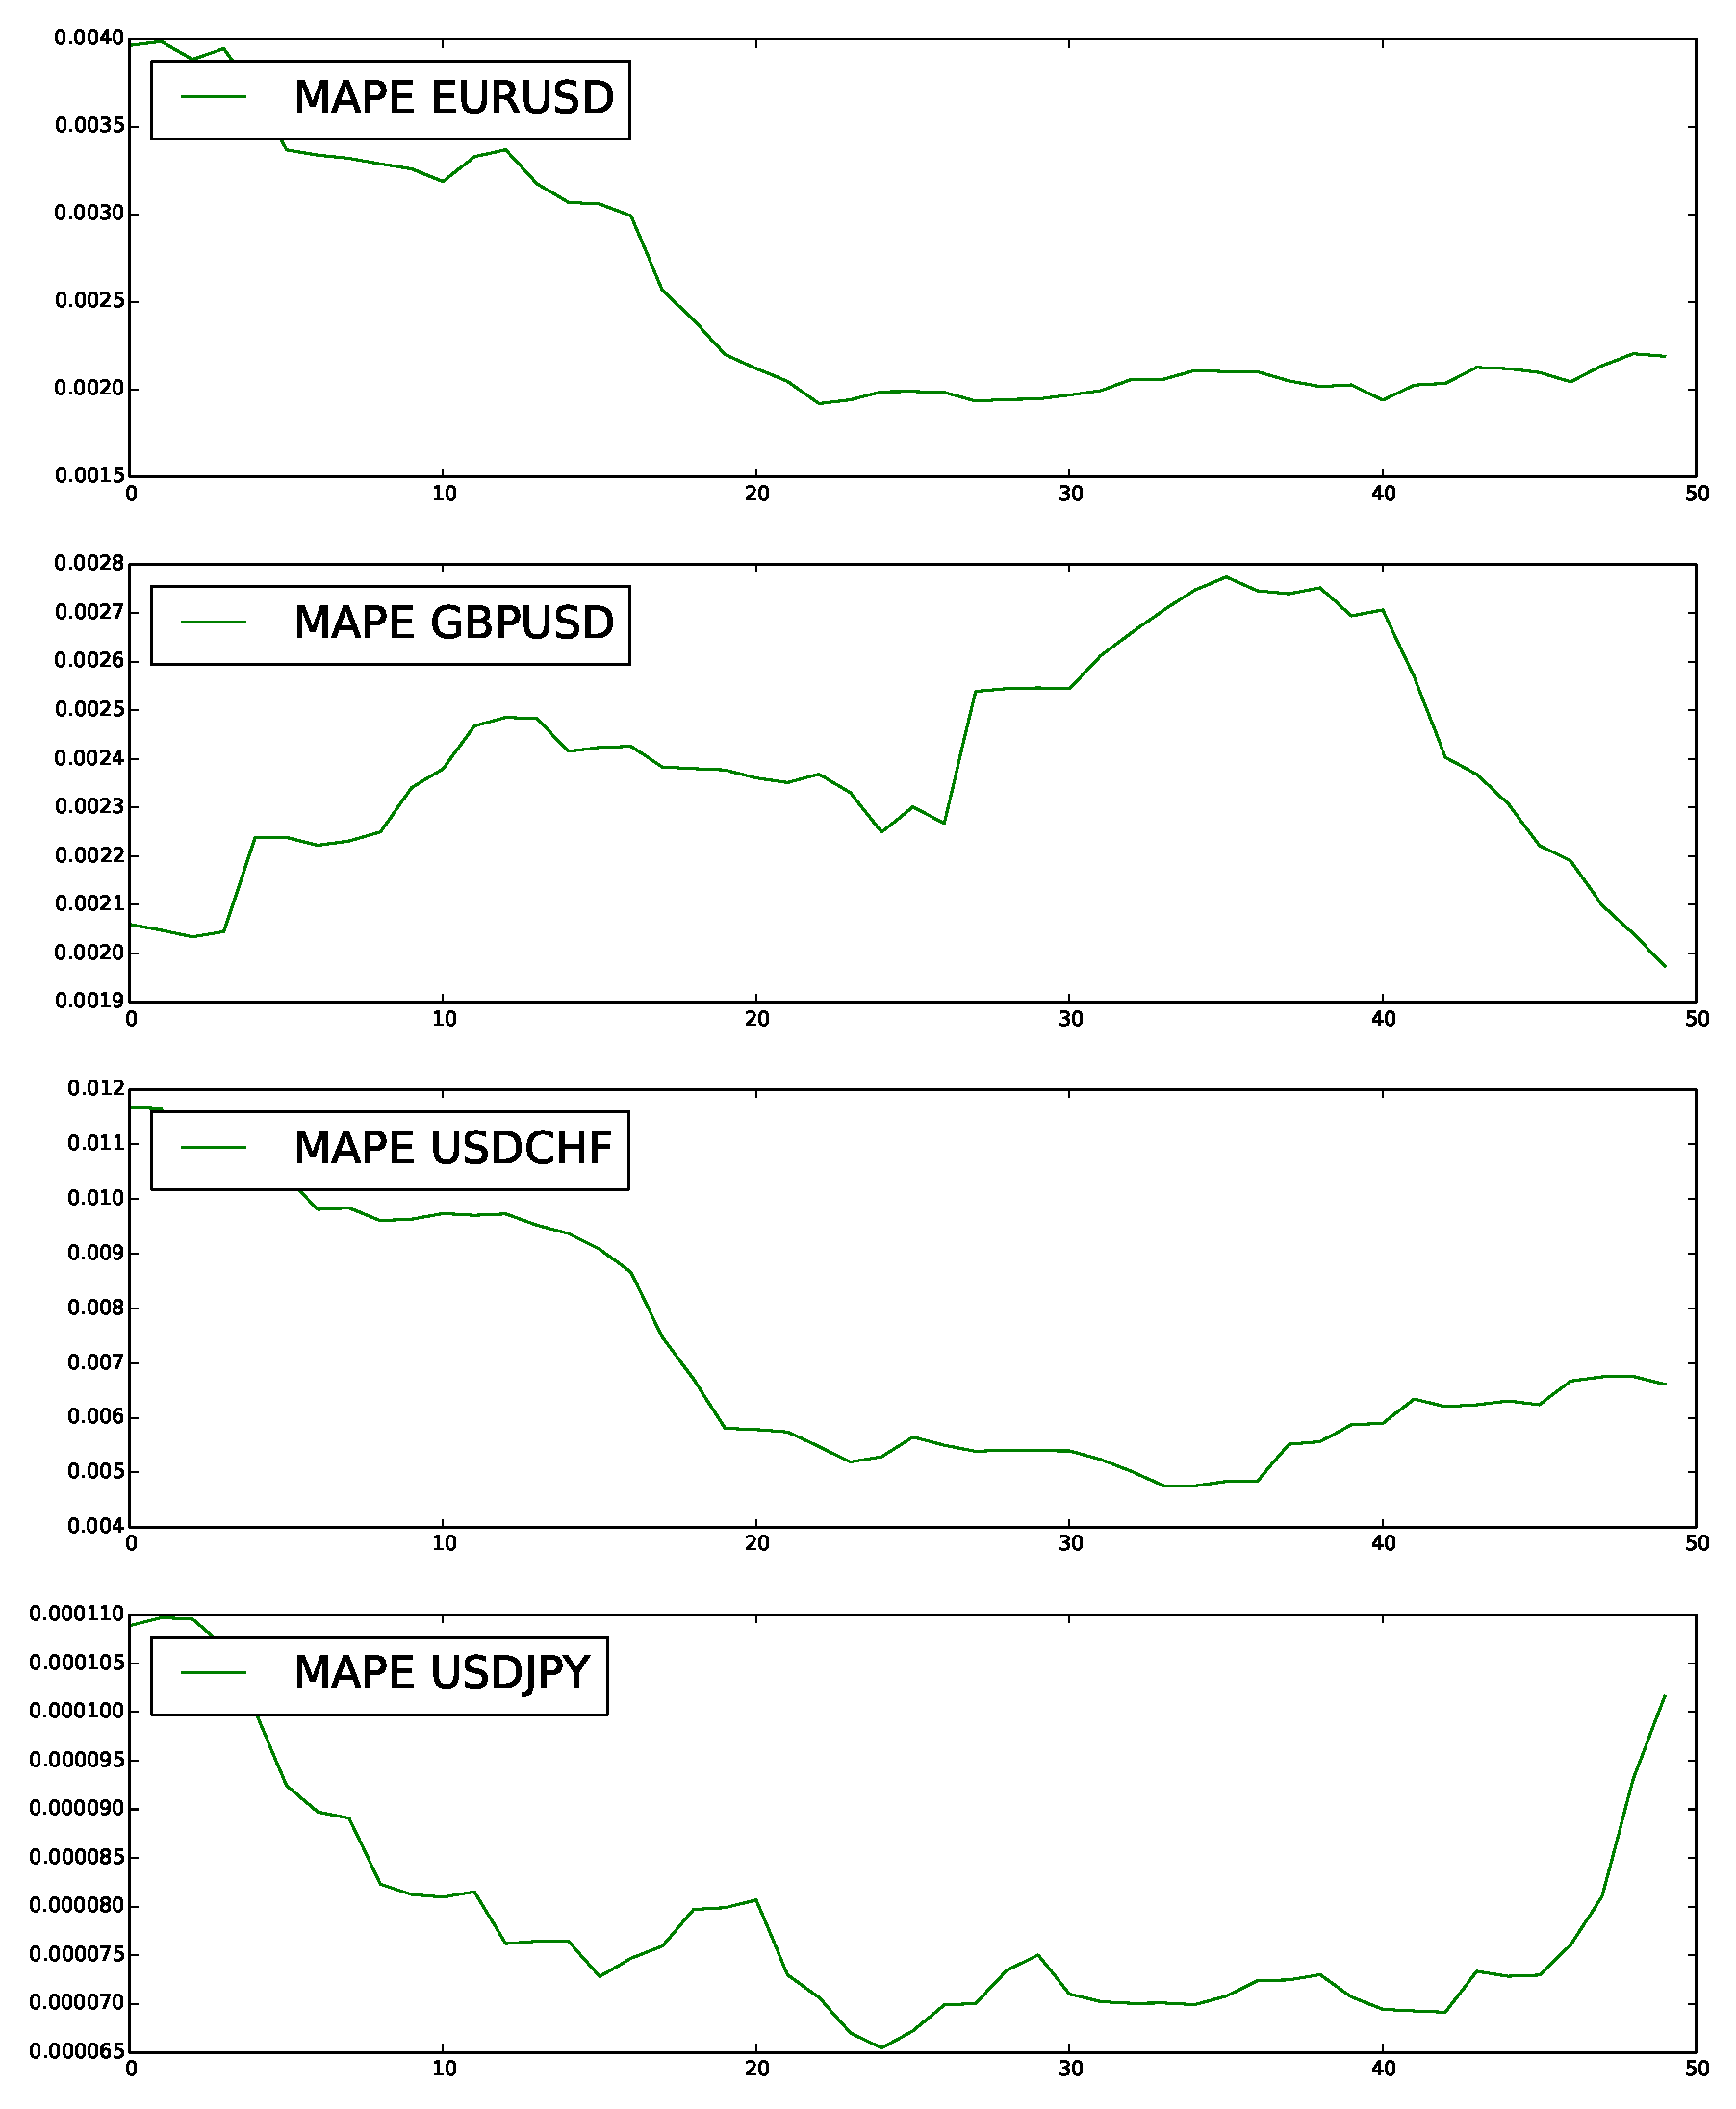
\includegraphics[width = 10.5cm]{img/mapes} 
  \caption{In-sample MAPEs example for 50 minutes. The average of them is
  considered to obtain new cointegration vectors.}
  \label{fig:mapes}
 \end{figure}



\subsection{Execution times} \label{sec:exectimes}
We ran OVECM and SLVECM 400 iterations. SLARIMA execution time is excluded
because its is not comparable with OVECM and SLVECM. SLARIMA was created based
on statsmodels library routine ARIMA.

The execution times are shown in the table~\ref{tab:extimes}.


\begin{table}[h!]
\caption{Execution times}
\label{tab:extimes}
\begin{center}
\begin{tabular}{|l|c|c|c|c|c|}
\hline
& $L$ & order & e  & Time[s] \\
\hline
OVECM & 100 &p=2  & 0      & 2.492\\
OVECM & 100 &p=2  & 0.0026  & 1.606\\
SLVECM & 100 &p=2& -- & 2.100\\
\hline
OVECM & 400 & p=5  & 0      & 3.513\\
OVECM & 400 &p=5  & 0.0041  & 2.569\\
SLVECM & 400 & p=5 & -- & 3.222\\
\hline
OVECM & 700 &p=3  & 0      & 3.296\\
OVECM & 700 &p=3  & 0.0032  & 2.856\\
SLVECM & 700 &p=3 & -- & 3.581\\
\hline
OVECM & 1000 & p=3 & 0      & 4.387\\
OVECM & 1000 & p=3  & 0.0022  & 2.408\\
SLVECM & 1000 & p=3  & -- & 3.609\\
\hline
\end{tabular}
\end{center}
\end{table}

It is clear that execution time depends directly on $L$ and $p$ since they
determine the size of matrix $\mathbf{A}$ and therefore affect the OLS function
execution time.
It is worthy of note that execution time also depends on mean\_error because it
determines how many times OVECM will recalculate cointegration vectors which is
an expensive routine.

Figure~\ref{fig:mapes} shows an example of the in-sample MAPE for 50 iterations.
When the average of the in-sample MAPEs is above mean\_error new cointegration
vectors are obtained. In consequence, OVECM performance increases when
mean\_error increases. However, this could affect accuracy, but
table~\ref{tab:stats} shows that using an appropriate mean\_error doesn't affect
accuracy considerable. 

\subsection{Performance accuracy} \label{sec:performacc}

Table~\ref{tab:stats} shows in-sample and out-of-sample performance measures:
MAPE, MAE and RMSE for OVECM, SLVECM and SLARIMA. Test were done using the
parameters defined in table \ref{tab:52params}.  We can see that OVECM has very
similar performance than SLVECM and this support the theory that cointegration
vectors vary little in time. Moreover, OVECM also out performed SLARIMA based on
these three performance measures. 


\begin{table*}[ht!]
\caption{Model measures}
\label{tab:stats}
\begin{center}
\tiny
\begin{tabular}{|l|l|c|c|c|c|c|c|c|c|}
\hline
\multicolumn{4}{|c|}{Model} & \multicolumn{3}{|c|}{In-sample} &
\multicolumn{3}{|c|}{Out-of-sample} \\ 
\hline
\hline
Method & $L$ & Parameters & e & 
MAPE & MAE& RMSE& 
MAPE & MAE& RMSE \\
\hline
 OVECM  &   100  &  P=2& 0.0026  &  0.00263&  0.00085&  0.00114&  0.00309&  0.00094&  0.00131\\
 OVECM  &   400  &  P=5& 0.0041  &  0.00378&  0.00095&  0.00127&  0.00419&  0.00103&  0.00143\\
 OVECM  &   700  &  P=3& 0.0032  &  0.00323&  0.00099&  0.00130&  0.00322&  0.00097&  0.00132\\
 OVECM  &   1000 &  P=3& 0.0022  &  
 \textbf{0.00175}&  \textbf{0.00062}&  \textbf{0.00087} &  
 \textbf{0.00172}&  \textbf{0.00061}&  \textbf{0.00090}\\
\hline
 SLVECM  &   100 &  P=2& -  &  0.00262&  0.00085&  0.00113&  0.00310&  0.00095&  0.00132\\
 SLVECM  &   400 &  P=5& -  &  0.00375&  0.00095&  0.00126&  0.00419&  0.00103&  0.00143\\
 SLVECM  &   700 &  P=3& -  &  0.00324&  0.00099&  0.00130&  0.00322&  0.00098&  0.00132\\
 SLVECM  &   1000 &  P=3& -  &  
 \textbf{0.00174}&  \textbf{0.00061}&  \textbf{0.00087}&  
 \textbf{0.00172}&  \textbf{0.00061}&  \textbf{0.00090}\\
\hline
SLARIMA & 100  &p,d,q=2,1,1 & - & 0.00285  &  0.00110  &  0.00308  &  0.00312  &0.00098  &  0.00144 \\
SLARIMA & 400  &p,d,q=1,1,1 & - & 0.00377  &  0.00101  &  0.00128  &  0.00418 & 0.00106 & 0.00145 \\
SLARIMA & 700  &p,d,q=2,1,1 & - & 0.00329  &  0.00102  &  0.00136  &  0.00324  & 0.00097  &  0.00133 \\
SLARIMA & 1000 &p,d,q=2,1,1 & - & \textbf{0.00281}  & \textbf{0.00074}  &  \textbf{0.00105}  &  \textbf{0.00177} & \textbf{0.00063}  &  \textbf{0.00092} \\
\hline
\end{tabular}
\end{center}
\end{table*}

We can also notice that in-sample performance in OVECM and SLVECM is related
with the out-of-sample performance.  This differs with SLARIMA which models with
good in-sample performance are not necessarily good out-of-sample models.
Moreover OVECM outperformed SLARIMA using the same window size.

Figure ~\ref{fig:accuracy} shows the out-of-sample forecasts made by our
proposal OVECM with the best parameters found based on table~\ref{tab:stats}
which follows the time series very well.  

\begin{figure}[h]
  \vspace{-0.2cm}
  \centering
   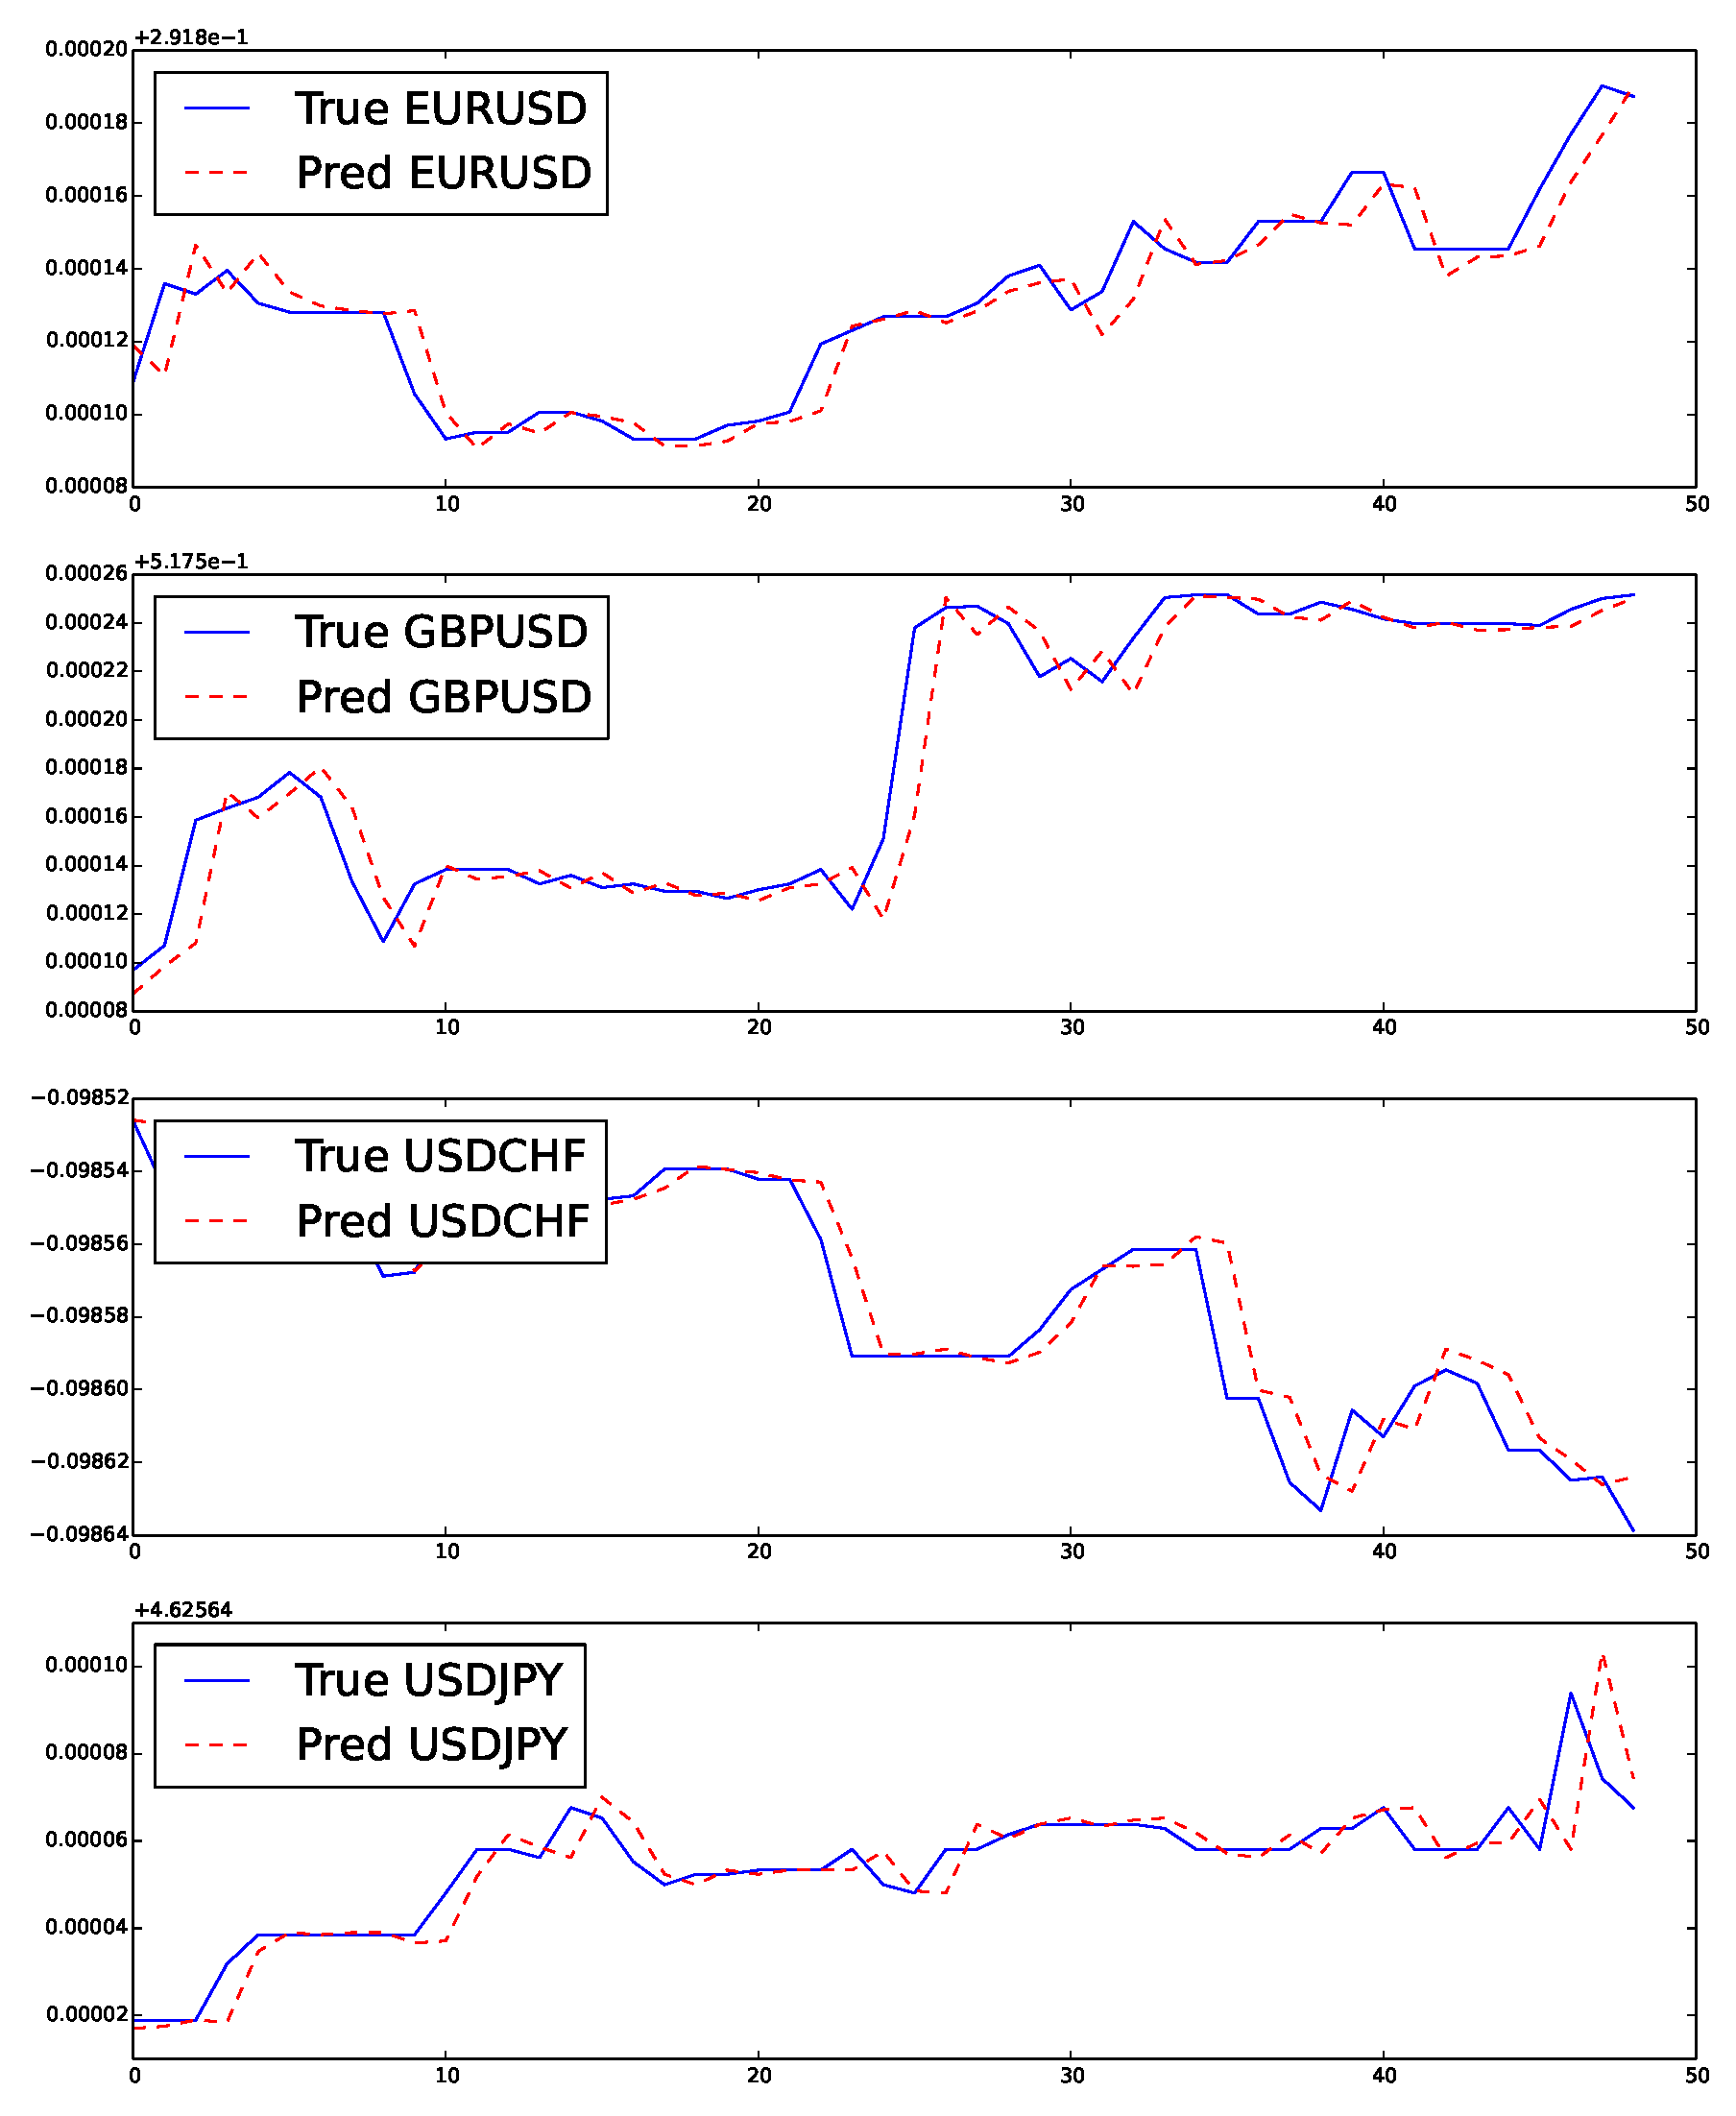
\includegraphics[width = 10cm]{img/accuracy} 
  \caption{OVECM forecasting accuracy example for 50 minutes using $L = 1000$ and $p =3$}
  \label{fig:accuracy}
 \end{figure}



\section{Conclusions} \label{sec:52conclusions}

A new online vector error correction method was presented. 
We have shown that our proposed OVECM considerably reduces execution times
without compromising solution accuracy.  OVECM was compared with VECM and ARIMA
with the same sliding window sizes and OVECM outperformed both in terms of
execution time. Traditional VECM slightly outperformed our proposal but the
OVECM execution time is lower.
This reduction of execution time is mainly because OVECM avoids the cointegration vector
calculation using the Johansen method. The condition for getting new vectors is
given by the mean\_error variable which controls how many times the Johansen method is
called. Additionally, OVECM introduces matrix optimisation in order to get the
new model in an iterative way.
We could see that our algorithm took much less than a minute at every
step. This means that it could also be used with higher frequency data and would
still provide responses before new data arrives.  

For future study, it would be interesting to improve the out-of-sample forecast
by considering more explicative variables, to increase window sizes or trying new
conditions to obtain new cointegration vectors. 

Since OVECM is an online algorithm which optimises processing time, it could be
used by investors as an input for strategy robots. Moreover, some technical
analysis methods could be based on its output. 


